% !TeX program = LuaLaTeX
\documentclass[12pt,oneside]{book}
\usepackage{comment} % enables the use of multi-line comments (\ifx \fi) 
\usepackage{lipsum} %This package just generates Lorem Ipsum filler text. 
\usepackage[left=0.5in,right=1.5in]{geometry}
\usepackage{amsmath}
\usepackage{amssymb,amsthm}  % assumes amsmath package installed
\newtheorem{theorem}{Theorem}
\newtheorem{corollary}{Corollary}
\usepackage{graphicx}
\usepackage{tikz}
\usetikzlibrary{arrows}
\usepackage{verbatim}
\usepackage{float}
\usepackage{tikz}
    \usetikzlibrary{shapes,arrows}
    \usetikzlibrary{arrows,calc,positioning}

    \tikzset{
        block/.style = {draw, rectangle,
            minimum height=1cm,
            minimum width=1.5cm},
        input/.style = {coordinate,node distance=1cm},
        output/.style = {coordinate,node distance=4cm},
        arrow/.style={draw, -latex,node distance=2cm},
        pinstyle/.style = {pin edge={latex-, black,node distance=2cm}},
        sum/.style = {draw, circle, node distance=1cm},
    }
\usepackage{xcolor}
\usepackage{mdframed}
\usepackage[shortlabels]{enumitem}
\usepackage{indentfirst}
\usepackage{hyperref}
\usepackage{mhchem}
\usepackage{titlesec}
\usepackage{fontspec}
\usepackage{titlesec, blindtext, color}
\usepackage{tcolorbox}
\usepackage{caption}
\usepackage{sidenotes} 
\usepackage{esdiff}
\renewcommand{\thesubsection}{\thesection.\alph{subsection}}
\usepackage{esvect}


\newtheorem{lemma}[theorem]{Lemma}

\newenvironment{problem}[2][Problem]
    { \begin{mdframed}[backgroundcolor=blue!8] \textbf{#1 #2} \\}
    {  \end{mdframed}}

% Define solution environment
\newenvironment{solution}
    {\textit{Solution:}}
    {}

\renewcommand{\qed}{\quad\qedsymbol}
\setlength\parindent{0pt}


\newcommand{\hsp}{\hspace{20pt}}
\titleformat{\chapter}[hang]{\Huge\bfseries}{\thechapter\hsp\textcolor[HTML]{0e4eb3}{\Huge|}\hsp}{0pt}{\Huge\bfseries}

\titleformat{\section}[hang]{\huge\bfseries}{\thesection\hsp\textcolor[HTML]{db3949}{\huge|}\hsp}{0pt}{\huge\bfseries}

%%%%%%%%%%%%%%%%%%%%%%%%%%%%%%%%%%%%%%%%%%%%%%%%%%%%%%%%%%%%%%%%%%%%%%%%%%%%%%%%%%%%%%%%%%%%%%%%%%%%%%%%%%%%%%%%%%%%%%%%%%%%%%%%%%%%%%%%
\begin{document}
\begin{titlepage}
    \newgeometry{left=7.5cm,top=1.2cm,right=1cm}
    \begin{tikzpicture}[remember picture, overlay]
    \node[opacity=1,inner sep=0pt] at (current page.center)
    {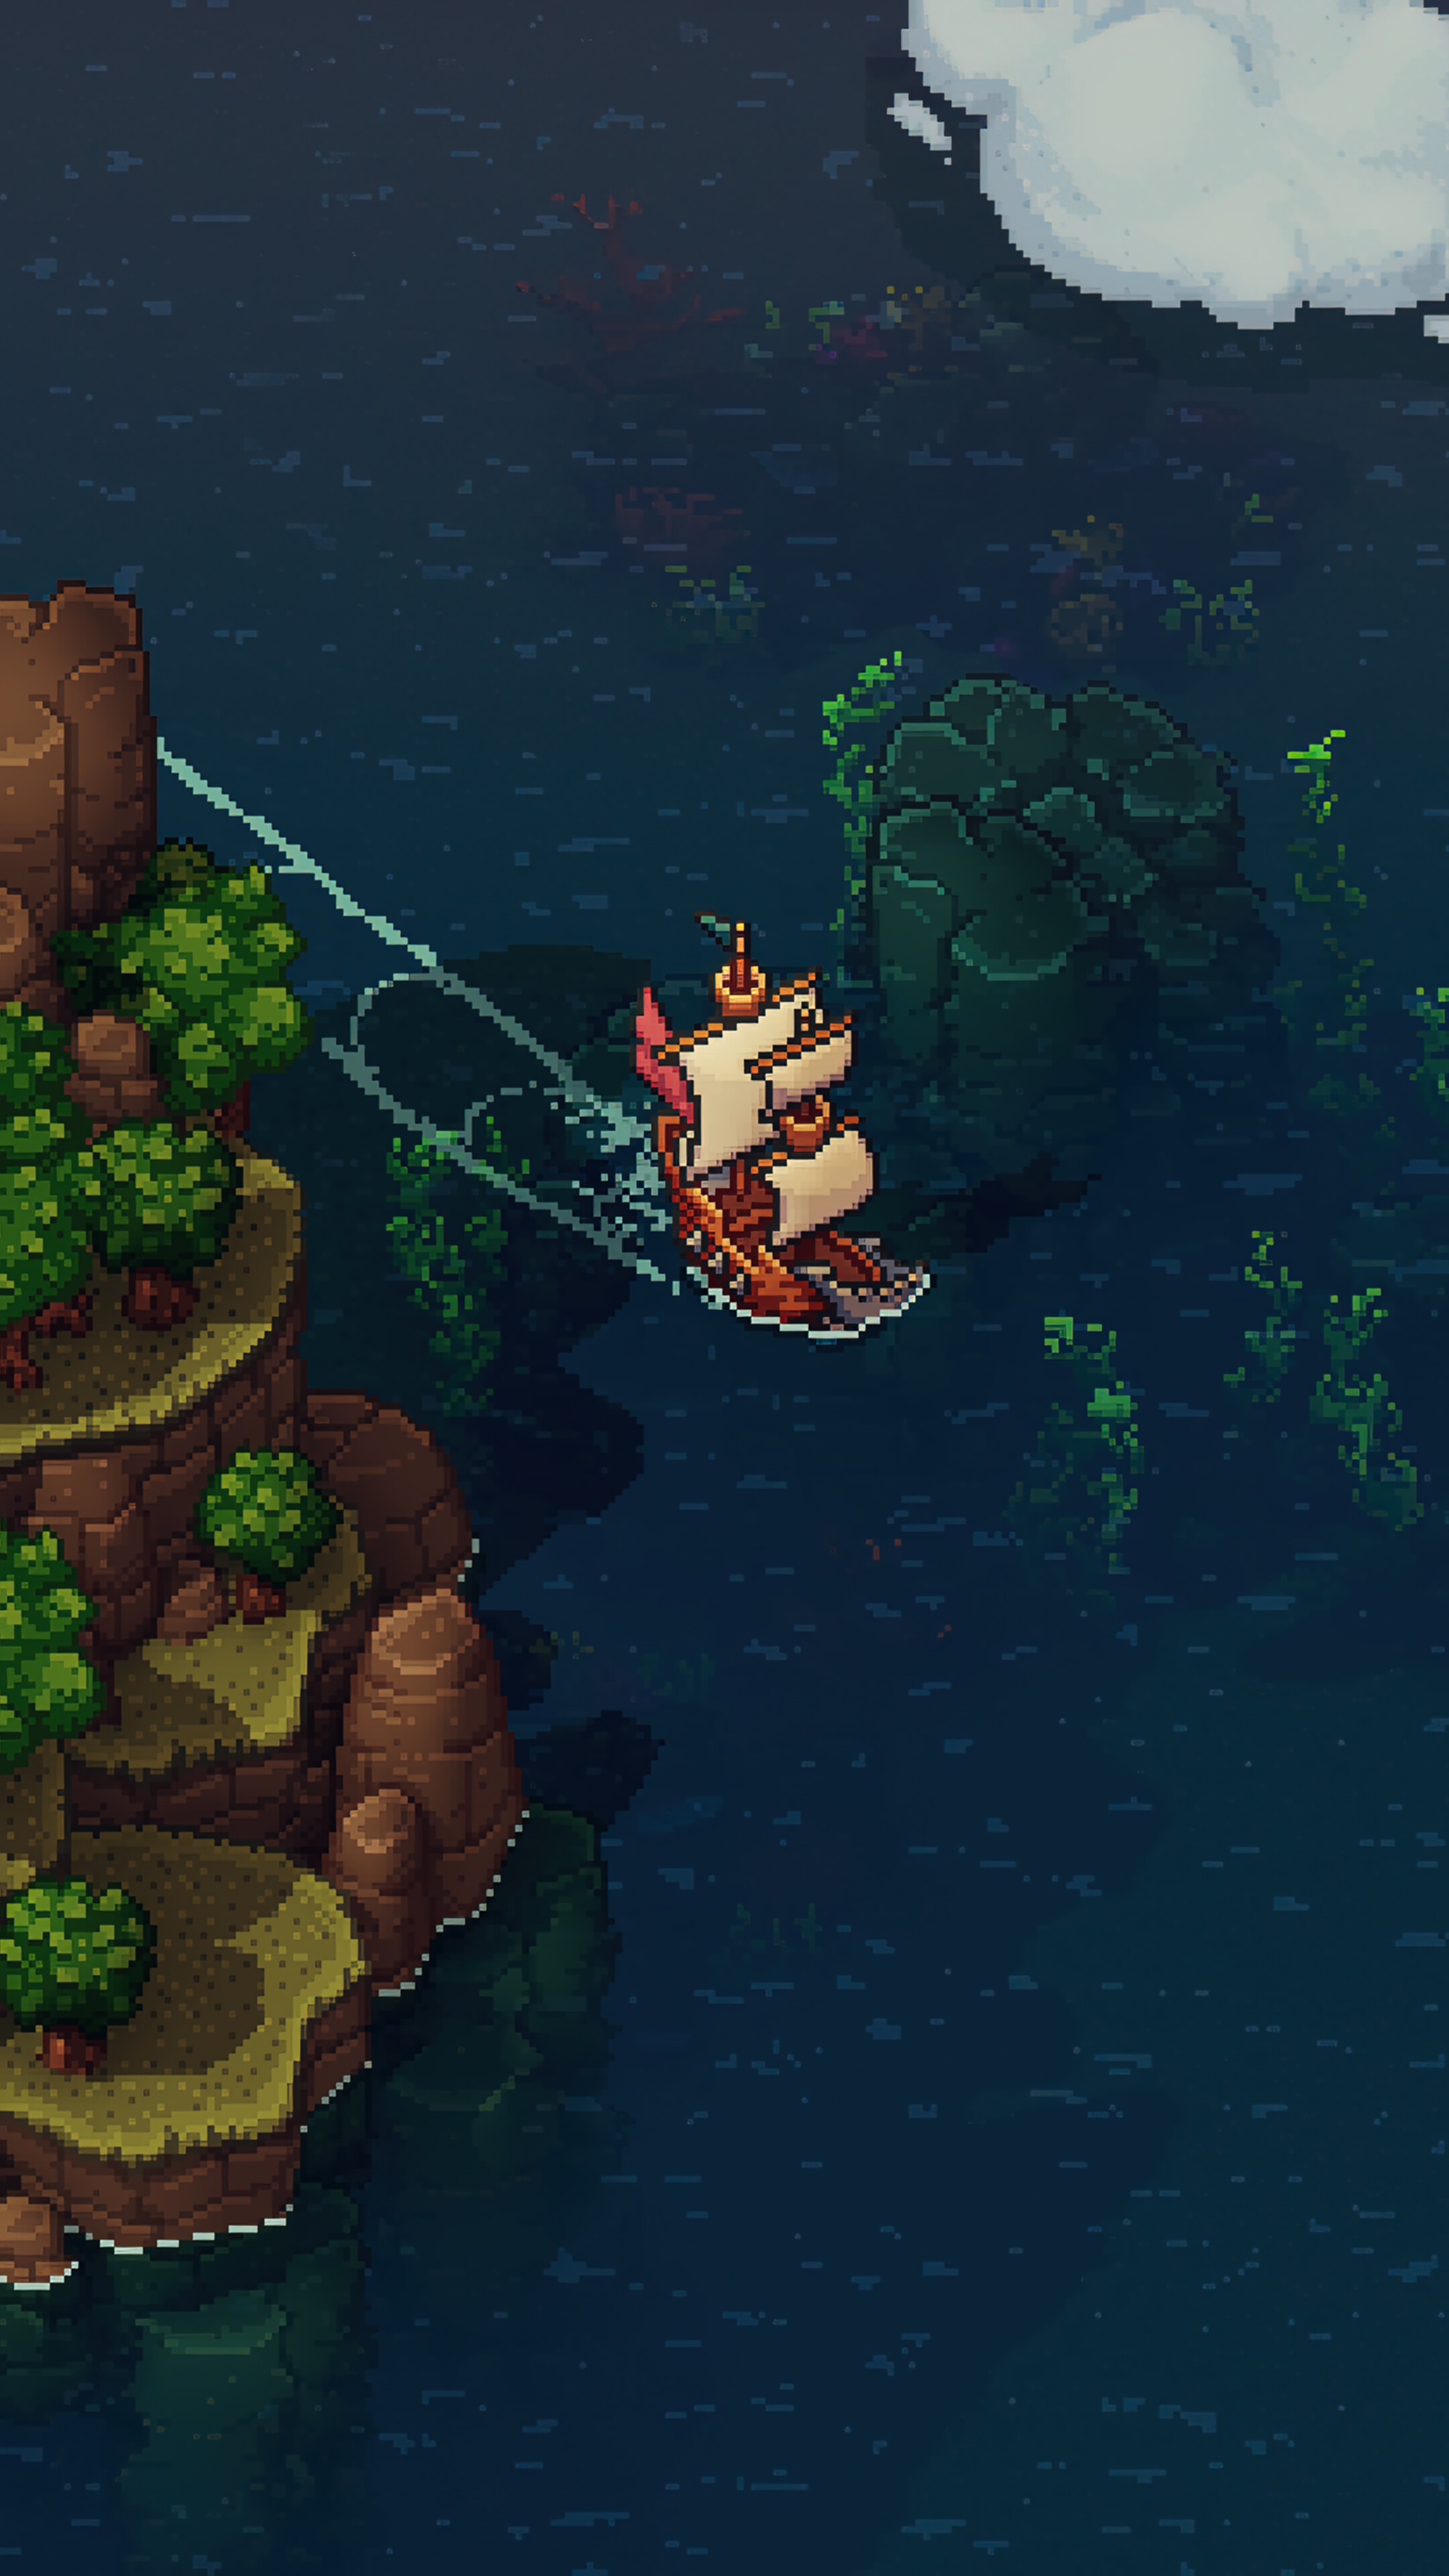
\includegraphics[width=\paperwidth,height=\paperheight]{graphics/cover.jpg}};
    \end{tikzpicture}
    \vphantom{A}
    \vfill
    \noindent{\fontsize{30}{30} \selectfont \bfseries\sffamily\noindent\textcolor{white}{Combinitorial Game Theory}}
    \\{\fontsize{20}{25} \selectfont \bfseries\sffamily \textcolor{white}{Aakash Ghosh}}
    \par
    \noindent
    \makebox[0pt][l]{\rule{1.3\textwidth}{1pt}}
    \par
    \noindent
    {\large\sffamily\textcolor{white}{Written with Fun}}
\end{titlepage}
\clearpage

%\setmainfont{KITTY CAT}
\setmainfont{Meows}

\tableofcontents

\chapter*{Preface}
This is a set of notes/book which I intend to write and maintain while doing my Master's  thesis. 


\part{Theory}
\chapter{Basic Stuff}
\section{Definitions}
\begin{marginfigure}%
    
\includegraphics[width=2.4\marginparwidth]{graphics/(10).png}
\end{marginfigure}
\begin{enumerate}
    \item \textbf{[Impartial Game]} are games in which both opponents have the same set of moves to make.
    \item \textbf{[Combinatorial games]} are two-player games with no hidden information and no chance elements
    \item \textbf{[Normal Play]} The player who makes the last move \textit{wins}.
    \item \item \textbf{[Misere Play]} The player who makes the last move \textit{loses}.
\end{enumerate}



\part{Game List}

\chapter{Impartial Games}
\section{Nim}


\begin{enumerate}
    \item \textbf{Setup}: Begin by arranging the piles of objects. The number of piles and the number of objects in each pile can vary, but traditionally, Nim is played with at least three piles.
  
    \item \textbf{Turn-Taking}: Players alternate turns, with one player going first. You can determine who goes first through a random selection or any other agreed-upon method.
  
    \item \textbf{Object Removal}: On each turn, a player must remove at least one object from one pile of their choice. The player can choose to remove any number of objects, but they must all come from the same pile.
  
    \item \textbf{Number of Piles}: The player can choose to remove objects from any one pile they wish, but they cannot take objects from multiple piles in a single turn.
  
    \item \textbf{Alternate Turns}: After a player makes their move, it becomes the other player's turn. Turns continue to alternate until the game ends.
  
    \item \textbf{End of the Game}: The game ends when all the objects have been removed from the last pile. The player who is forced to remove the last object from the last pile loses the game.
  
    \item \textbf{Winning Strategy}: Nim has a mathematical strategy that guarantees a win if executed correctly. This strategy involves creating a winning position by maintaining a specific pattern of objects in the piles. A player can force their opponent into a losing position by following this strategy.
  \end{enumerate}


\subsection{Strategy}
We define $\oplus$ as the XOR operation. For heaps $H_1,H_2...H_n$ containing $\alpha_1,\alpha_2..\alpha_n$ coins, we define the nim-sum of the game as $\oplus_{i=1}^n\alpha_n$. Note that at winning position, the last player, makes the nim-sum zero. 
\begin{lemma}
    If $G=H_1+H_2\hdots H_n$ has a nim-sum zero then any legal maove makes the nim-sum non-zero 
\end{lemma}
\begin{proof}
    Assume that $\mathcal{N}$ acts on heap $H_i$ changing $\alpha_i$ to $\beta_i$. Then:
    \begin{align*}
        \text{Nim-Sum}=&\alpha_1\oplus\alpha_2..\oplus\beta_i\oplus..\alpha_n\\
        =&(\alpha_1\oplus\alpha_2..\oplus\beta_i\oplus..\alpha_n)\oplus(\alpha_1\oplus\alpha_2..\oplus\alpha_i\oplus..\alpha_n)\quad[\text{As initial nim-sum was zero}]\\
        =&(\alpha_1\oplus\alpha_1)\oplus(\alpha_2\oplus\alpha_2)...(\alpha_i\oplus\beta_i)...(\alpha_n\oplus\alpha_n)\\
        =&(\alpha_i\oplus\beta_i)\quad[\text{As $x\oplus x=0$}]
    \end{align*}
    As $\alpha_i\ne0$ and $\beta_i\ne \alpha_i$ there exists some bit in the binary expression that changes. Therefore, the new nim-sum is non zero.
\end{proof}
\begin{lemma}
    If $G=H_1+H_2\hdots H_n$ and $G$ has a non-zero nim-sum, then $\mathcal N$ has a move by which he makes the nim-sum zero.
\end{lemma}
\begin{proof}
    Let $G$ have nim-sum $s$, Let $s$ have $k$ significant digits. Find $\alpha_i$ which has 1 in the $k^{th}$ place. Set $\alpha_i'=s\oplus\alpha_i$. Note that from $k+1^{th}$ significant digit, $\alpha_i$ and $\alpha_i'$ are the same. On the $k^{th}$ digit, $\alpha_i'$ is 0 while $\alpha_i$ is 1. Therefore, $\alpha_i'<\alpha_i$. Now note if $\alpha_i$ is replaced with $\alpha_i'$ then the new nim-sum is $\alpha_1\oplus\alpha_2\hdots \alpha_i\oplus s\hdots \alpha_{n-1}\oplus\alpha_n=s\oplus s=0$ 
\end{proof}

By th above argument it is clear if $G$ has non-zero nim-sum, $\mathcal{N}$ has winning strategy, else $\mathcal{P}$ has winning strategy


\subsection{Mirroring on two heaps}
If $G=H_1\oplus H_2$ where $\alpha_1= \alpha_2$, then $\mathcal P$ has a winning strategy by mirroring $\mathcal N$. For every move by $\mathcal N$, $\mathcal P$ makes the same move but on the other heap. Therefore, it is guaranteed $\mathcal P$ has a move after every move of $\mathcal N$, and therefore, the last move is always made by $\mathcal P$.



\section{Dawson's Kayles}
\begin{enumerate}
    \item \textbf{Setup}: Start with a finite number of rows of pins or pegs arranged in any pattern. The number of pins and the initial arrangement can vary.
  
    \item \textbf{Turn-Taking}: Players alternate turns, with one player going first. You can determine who goes first through a random selection or any other agreed-upon method.
  
    \item \textbf{Move}: On each turn, a player takes two consecutive pins.
  
    \item \textbf{Alternate Turns}: After a player makes their move, it becomes the other player's turn. Turns continue to alternate until the game ends.
  
    \item \textbf{End of the Game}: The game ends when no two consecutive pins remain.
    
    \item \textbf{Strategy}: No optimal strategy is known.
\end{enumerate}

\begin{figure}[ht]
    \centering
    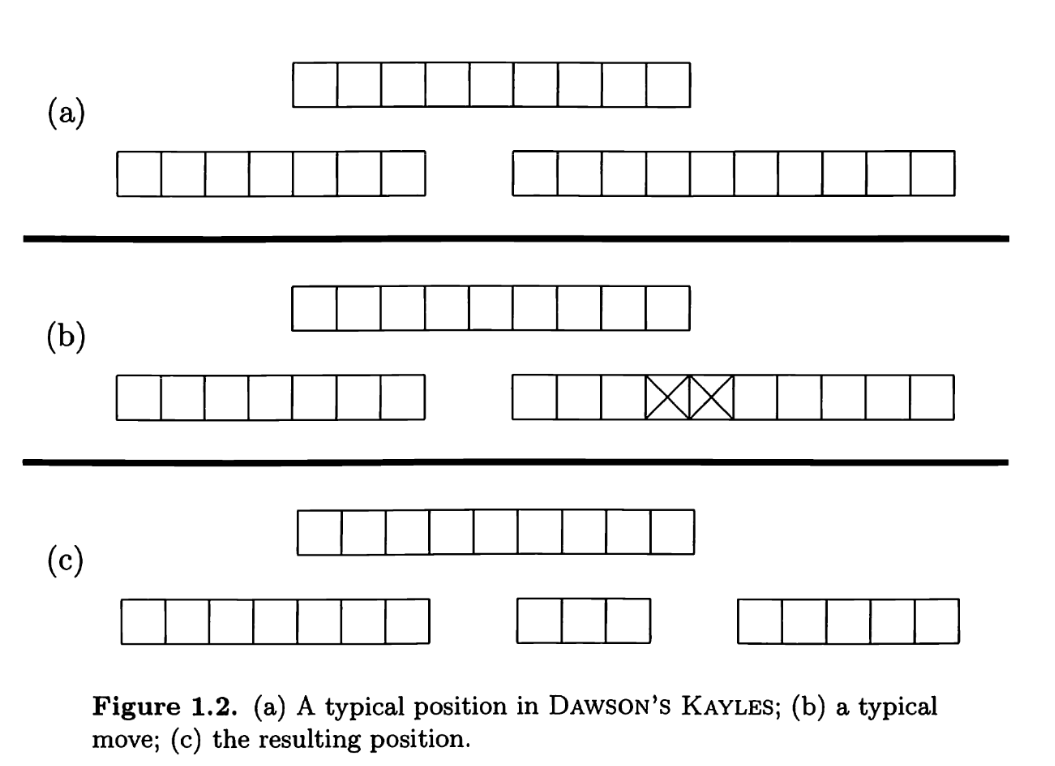
\includegraphics[width=0.8\textwidth]{graphics/dk.png}
\end{figure}







\chapter{Partizian games}
\section{Hackenbush}
\begin{enumerate}
    \item \textbf{Setup}: Start with a graph composed of edges and vertices. Each edge represents a colored segment, and each vertex represents a connection point. A vertex is denoted as the ground
  
    \item \textbf{Turn-Taking}: Players alternate turns, with one player going first. You can determine who goes first through a random selection or any other agreed-upon method.
  
    \item \textbf{Move}: At Left's move, left removes an edge of color blue or green. At red's move, red removes an edge of color red or green. If removing an edge  disconnects a graph, the component not connected to the ground is deleted.
  
    \item \textbf{End of the Game}: The game ends when no more edges (colored segments) are left in the graph. The player who removes the last edge or edges is declared the winner.
  
    \item \textbf{Optional Rule}: In some variations, there may be edges which can be removed by both players.
\end{enumerate}
\section{Domineering}


\begin{enumerate}
    \item \textbf{Board Setup}: Start with an empty grid board of dimensions $m \times n$(Generally $8\times 8$). The board consists of cells that can be either empty or occupied by a domino. Each domino occupies two adjacent cells horizontally or vertically.
  
    \item \textbf{Player Assignments}: Two players participate in the game, traditionally named Vertical and Horizontal. Vertical player can only place dominoes vertically, and Horizontal player can only place dominoes horizontally.
  
    \item \textbf{Turn-Taking}: Players alternate turns, with Vertical player going first. 
  
    \item \textbf{Domino Placement}: On each turn, the current player must place a domino on the board. The domino must fit within the bounds of the board and cannot overlap or cross any existing dominoes.
  
    \item \textbf{Number of Dominos}: Each player must place exactly one domino on their turn. If a player cannot make a legal move, they must pass their turn.
  
    \item \textbf{Alternate Turns}: After a player makes their move or passes, it becomes the other player's turn. Turns continue to alternate until the game ends.
  
    \item \textbf{End of the Game}: The game ends when no player can make a legal move. The player who cannot make a legal move loses the game.
  
    \item \textbf{Winning Condition}: The player who loses is the one unable to make a legal move, meaning their opponent has effectively blocked their available positions.
  
  \end{enumerate}


\end{document}










